The original drone from \cite{thingiverse_rpi_drone} includes only a simple body with a peg-in-hole mounting system
for the legs.
The legs are symmetrical for interchangeability and design ease.
This design retains the body and legs from the original drone with some additions.

The first addition to the original drone is a small tilt gimbal
(shown in Figures \ref{figure:tilt_gimbal_base} and \ref{figure:tilt_gimbal_camera_mount}),
that is mounted on the front of the drone.
The tilt gimbal includes a mount for a standard Raspberry Pi camera module and a space for a micro servo that serves
as the gimbal's actuator.
Its rotational axis is supported by a single screw and the rotational axis of the micro servo.
The camera module is attached with screws, and its ribbon cable extends upwards above the drone body.
The gimbal base is aligned with the

\begin{figure}
    \centering
    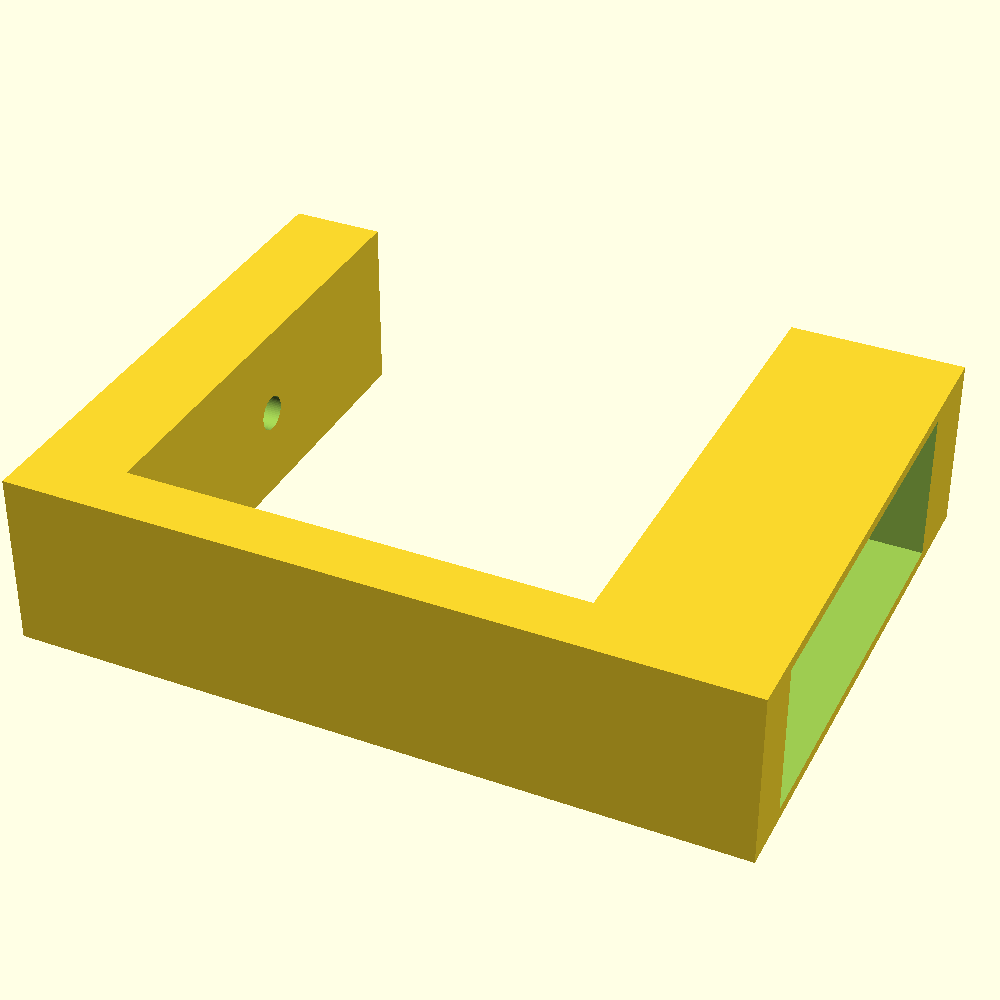
\includegraphics[width=0.75\columnwidth]{images/gimbal_base.png}
    \caption{The tilt gimbal base.}
    \label{figure:tilt_gimbal_base}
\end{figure}

\begin{figure}
    \centering
    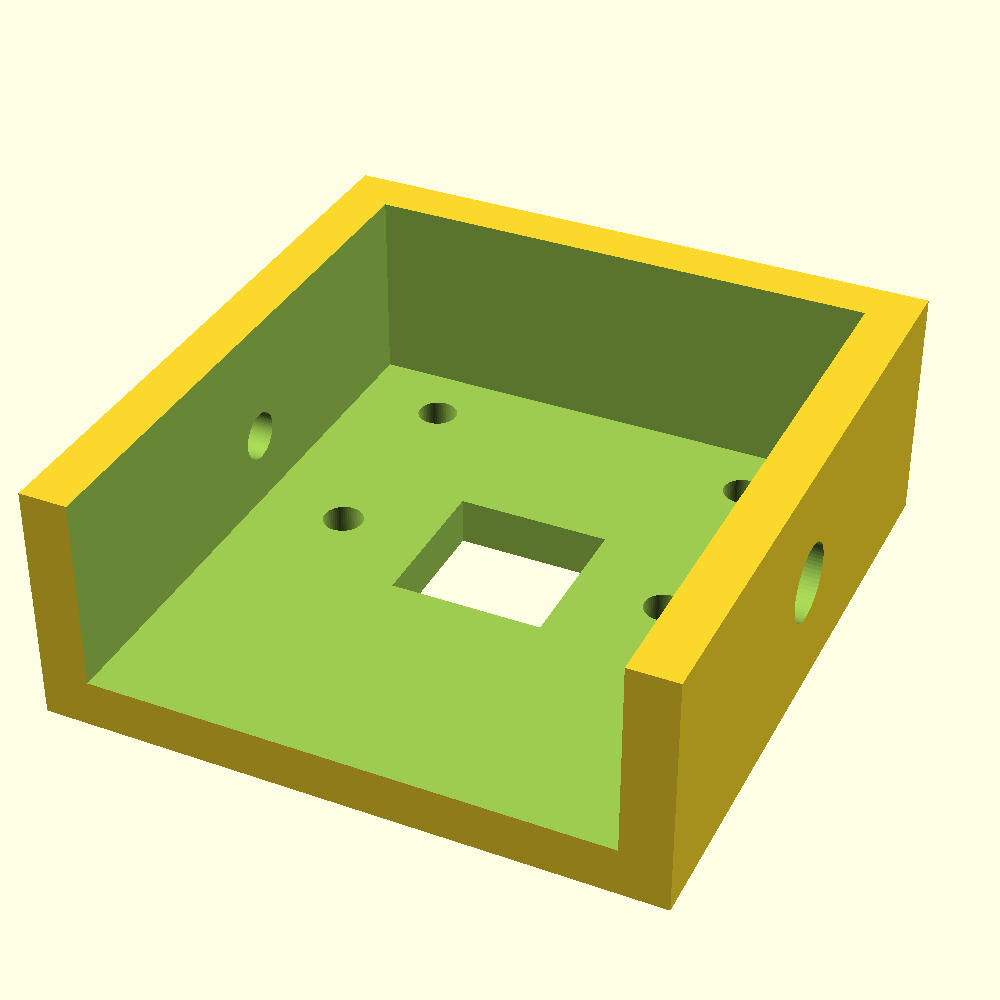
\includegraphics[width=0.75\columnwidth]{images/gimbal_camera_mount.png}
    \caption{The tilt gimbal camera mount.}
    \label{figure:tilt_gimbal_camera_mount}
\end{figure}

The second addition is a set of mounts for the drone's electronic speed controllers.
The speed controllers fit into slots on the drone's body and are held in place simply with electrical tape.
The design also includes mounting holes for the Raspberry Pi, power distribution board,
and legs for quick and reliable assembly.

The drone body is flat on its top side (except for conical indentations that allow the leg screws to sit flush), so that
it can be easily 3D printed upside down.
The drone body is shown in Figure \ref{figure:drone_body}.

\begin{figure}
    \centering
    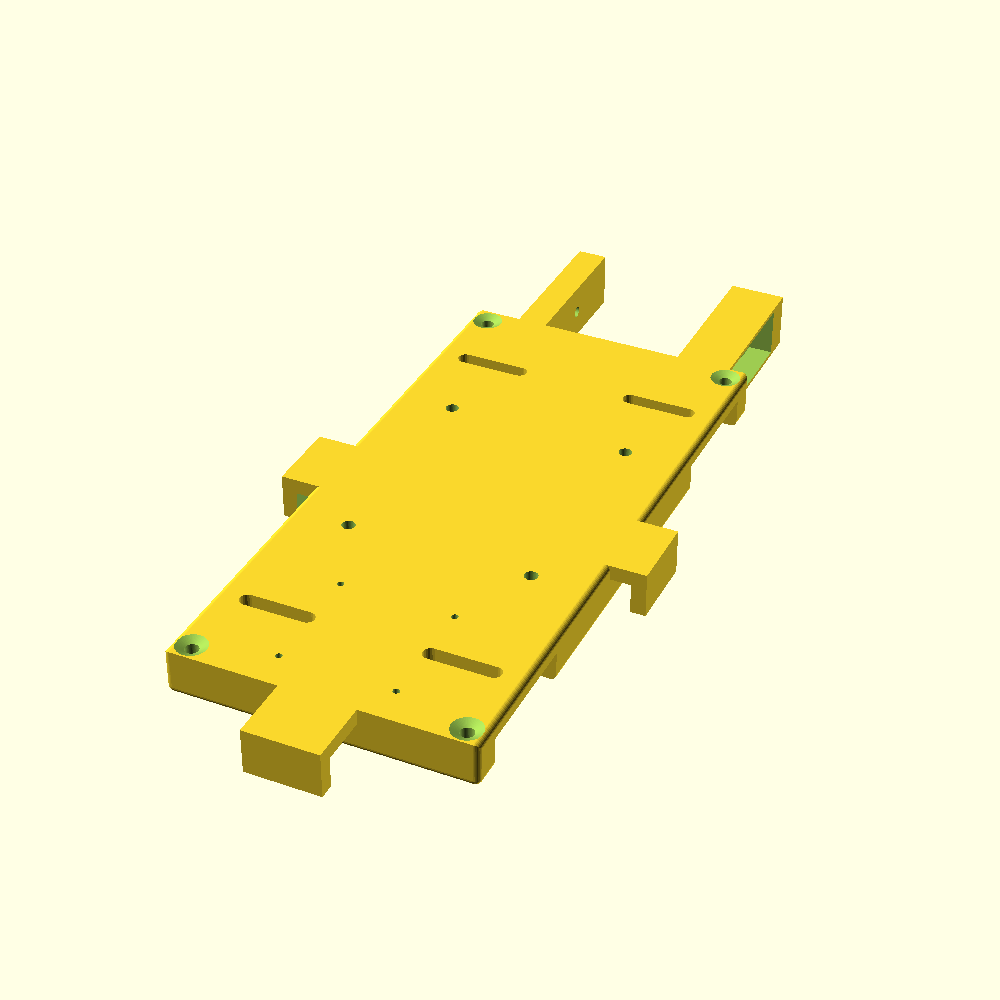
\includegraphics[width=\columnwidth]{images/body.png}
    \caption{The drone body with attached gimbal mount.}
    \label{figure:drone_body}
\end{figure}

Finally, an ``upper deck'' (shown in Figure \ref{figure:upper_deck}) provides additional component mounting space.
It attaches to the holes for the Raspberry Pi and provides a flat area above the Raspberry Pi, as well as a hole for the
cords that connect the components to the computing system.

\begin{figure}
    \centering
    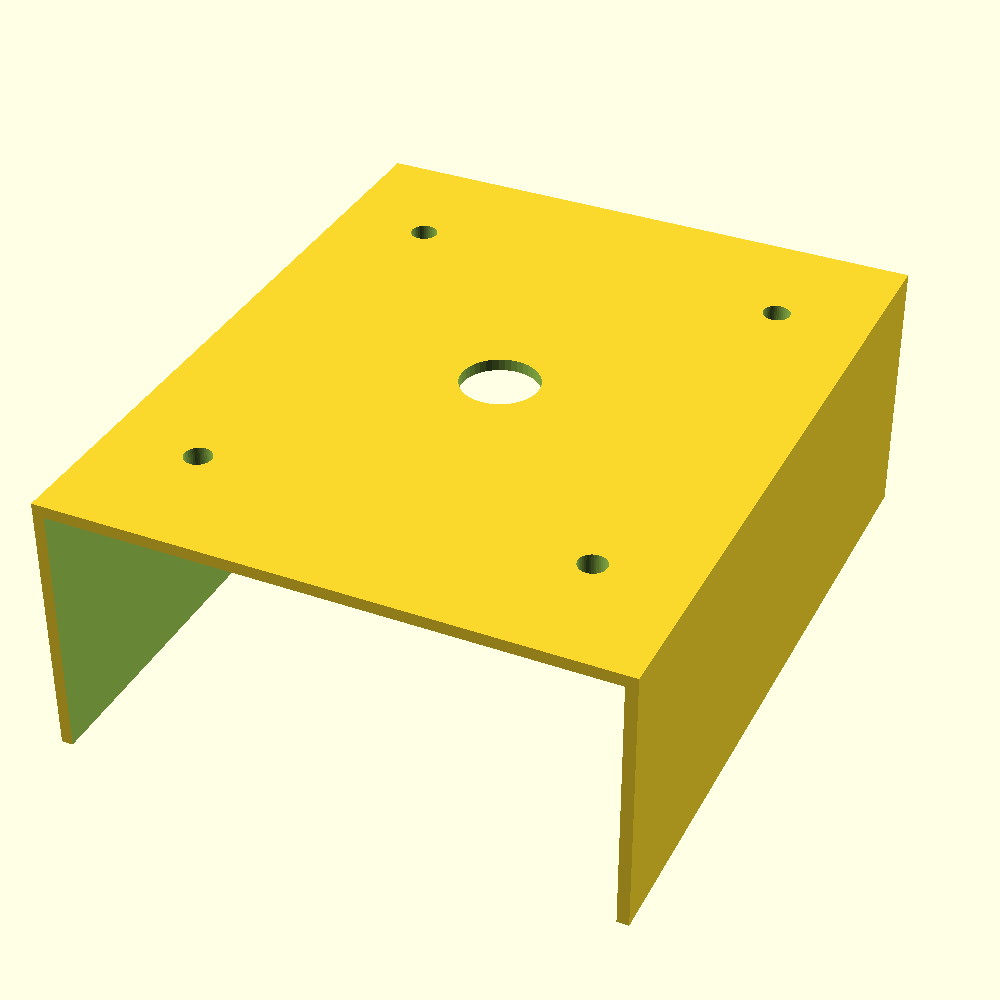
\includegraphics[width=\columnwidth]{images/upper_deck.png}
    \caption{Upper deck.}
    \label{figure:upper_deck}
\end{figure}